\documentclass[11pt]{article}
\usepackage[utf8]{inputenc}
\usepackage{polski}
\usepackage{graphicx}
\usepackage{array}
\usepackage{paralist}
\usepackage{verbatim}
\usepackage{subfig}
\usepackage{amsmath}
\usepackage{float}
\usepackage{amsthm}
\usepackage{amssymb}
\usepackage{pdfpages}
\usepackage{amsfonts}
\usepackage{tikz}
\usepackage{wasysym}
\usepackage[linguistics]{forest}
\usetikzlibrary{shapes,backgrounds}
\usepackage[margin=1in]{geometry}
\setlength\parindent{0pt}
\theoremstyle{definition}
\newtheorem{zadanie}{Zadanie}
% \numberwithin{zadanie}{subsection}
\DeclareRobustCommand{\stirling}{\genfrac\{\}{0pt}{}}
\renewcommand*{\proofname}{Rozwiązanie}
\newtheorem{theorem}{Twierdzenie}
\title{Grafy i sieci}
\author{Igor Nowicki}
\begin{document}
\maketitle

\section{Definicje i twierdzenia}

\textbf{Graf pochodny grafu skierowanego $G = (V,E)$} to taki graf nieskierowany $G' = (V, E')$, gdzie krawędź pomiędzy wierzchołkami $a,b$ należy do $E'$ wtedy i tylko wtedy, gdy do $E$ należy krawędź od $a$ do $b$ lub od $b$ do $a$.

Intuicyjnie - graf pochodny grafu skierowanego to ten sam graf, tylko z krawędziami bez wyszczególnionych kierunków.

\textbf{Grafem spójnym} nazywamy graf spełniający warunek, że dla każdej pary wierzchołków istnieje ścieżka która je łączy.

\textbf{Cyklem} nazywamy każdą drogę zamkniętą w grafie, tj. taką której wierzchołek końcowy jest tożsamy z wierzchołkiem początkowym.

\textbf{Cykl Eulera grafu $G$} to taki cykl w grafie który przechodzi przez wszystkie krawędzie dokładnie raz. Jeśli dany graf umożliwia na stworzenie cyklu Eulera, to taki graf nazywa się \textit{grafem eulerowskim}.

Warunkiem koniecznym i wystarczającym na to by spójny graf nieskierowany był eulerowski jest parzystość stopni wszystkich wierzchołków. Natomiast warunkiem w spójnym grafie skierowanym jest taka sama liczba krawędzi wchodzących i wychodzących dla każdego wierzchołka.



\begin{proof}

\end{proof}

\section{Zadania na kolokwium}

\begin{zadanie}
    \begin{enumerate}
        \item Czy istnieje graf skierowany $G$, który ma cykl Eulera, ale którego graf pochodny $PG$ nie ma cyklu Eulera?
        \item Niech $G$ będzie grafem skierowanym. Wiemy, że w $G$ istnieje cykl Eulera. Czy graf musi być silnie spójny? Jeśli musi - udowodnij to. Jeśli nie musi - podaj przykład odpowiedniego grafu.
    \end{enumerate}
\end{zadanie}
\begin{proof}
    \begin{enumerate}
        \item

              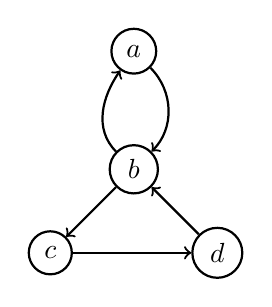
\begin{tikzpicture}[node distance={15mm}, thick, main/.style = {draw, circle}]
                  \node[main] (1) {$a$};
                  \node[main] (2) [below of=1] {$b$};
                  \node[main] (3) [below left of=2] {$c$};
                  \node[main] (4) [below right of=2] {$d$};
                  \draw[->] (1) to [out=315,in=45,looseness=1] (2);
                  \draw[->] (2) to [out=135,in=235,looseness=1] (1);
                  \draw[->] (2) to (3);
                  \draw[->] (3) to (4);
                  \draw[->] (4) -- (2);
              \end{tikzpicture} przekształca się do:
              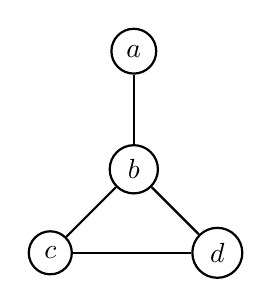
\begin{tikzpicture}[node distance={15mm}, thick, main/.style = {draw, circle}]
                  \node[main] (1) {$a$};
                  \node[main] (2) [below of=1] {$b$};
                  \node[main] (3) [below left of=2] {$c$};
                  \node[main] (4) [below right of=2] {$d$};
                  \draw(1) to (2);
                  \draw(2) to (3);
                  \draw(3) to (4);
                  \draw (4) to (2);
              \end{tikzpicture}. Pierwszy graf jest eulerowski ($d^- = d^+$ dla każdego wierzchołka), drugi nie (wierzchołki $a$ oraz $b$ mają nieparzystą liczbę krawędzi).

        \item Jeśli graf skierowany jest eulerowski, oznacza to że z każdego wierzchołka można dotrzeć do dowolnego innego wierzchołka. Zatem z założenia graf \textbf{musi być} silnie spójny.
    \end{enumerate}

\end{proof}

\begin{zadanie}

    Graf nieskierowany $G=(V,E)$ zdefiniowany jest następująco: zbiór wierzchołków $V=\{1,2,...,10\};$ zbiór krawędzi $E=\{\{i,j\};i=1,...,9;j=i+1\}\cup\{10,1\}\cup\{8,4\}$.

    \begin{enumerate}
        \item Czy ten graf ma drogę Eulera? Uzasadnij. Jeśli tak, to jaką długość ma ta droga?
        \item Czy ten graf ma cykl Eulera? Uzasadnij. Jeśli nie ma cyklu Eulera, dodaj jak najmniejszą liczbę krawędzi, aby w grafie istniał cykl Eulera.
    \end{enumerate}
\end{zadanie}
\begin{proof}
    \begin{enumerate}
        \item Warunek na występowanie drogi Eulera w grafie nieskierowanym jest taki, by wszystkie wierzchołki poza dwoma były parzystego rzędu. W grafie wierzchołki 8 oraz 4 mają rząd nieparzysty (3), pozostałe mają rząd parzysty, 2. Zatem droga Eulera powinna przebiegać pomiędzy wierzchołkami 8 a 4. Długość drogi będzie oczywiście równa liczbie krawędzi, czyli 11.
        \item Graf nie ma cyklu Eulera, ponieważ jego dwa wierzchołki są nieparzyste. Można to rozwiązać poprzez dodanie jeszcze trzech krawędzi, np: od 8 do 3, od 4 do 9, oraz od 3 do 9.
    \end{enumerate}

\end{proof}
\begin{zadanie}

    $$ M = \left( \begin{matrix} 0 & 1 & 1 & 0 & 0 & 0 \\ 1 & 0 & 1 & 0 & 0 & 1 \\ 0 & 1 & 0 & 0 & 0 & 1 \\ 0 & 0 & 0 & 0 & 1 & 0 \\ 0 & 1 & 1 & 1 & 0 & 0 \\ 1 & 0 & 0 & 0 & 1 & 0 \end{matrix} \right) $$

    $M$ jest macierzą sąsiedztwa grafu skierowanego $G$.

    \begin{itemize}
        \item Czy $G$ ma cykl Eulera?
        \item Czy $G$ ma drogę Eulera?
        \item Jeśli $M$ ma cykl (drogę) Eulera - wskaż ten cykl (drogę).
        \item Jesli nie ma, dodaj jak najmniej łuków, aby zmodyfikowany graf miał drogę (cykl) Eulera. Uzasadnij konstrukcję.
    \end{itemize}

\end{zadanie}
\begin{proof}
    Rysunek grafu:

    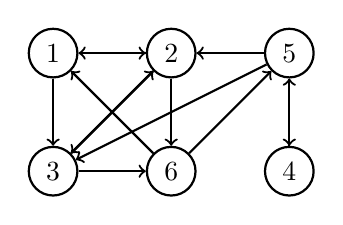
\begin{tikzpicture}[node distance={15mm}, thick, main/.style = {draw, circle}]
        \node[main] (1) {$1$};
        \node[main] [right of=1] (2) {$2$};
        \node[main] [below of=1] (3) {$3$};
        \node[main] [right of=2] (5) {$5$};
        \node[main] [below of=5] (4) {$4$};
        \node[main] [right of=3] (6) {$6$};
        \draw[->] (1) to (2);
        \draw[->] (1) to (3);
        \draw[->] (2) to (1);
        \draw[->] (2) to (3);
        \draw[->] (2) to (6);
        \draw[->] (3) to (2);
        \draw[->] (3) to (6);
        \draw[->] (4) to (5);
        \draw[->] (5) to (2);
        \draw[->] (5) to (3);
        \draw[->] (5) to (4);
        \draw[->] (6) to (1);
        \draw[->] (6) to (5);
    \end{tikzpicture}

    Graf jest (słabo) spójny. Widzimy, że wierzchołki mają następujące rzędy (możemy je policzyć poprzez liczenie jedynek odpowiednio w n-tej rzędzie i n-tej kolumnie):

    \begin{enumerate}
        \item $d(1)^+ = 2, d(1)^-=2$,
        \item $d(2)^+ = 3, d(2)^-=3$,
        \item $d(3)^+ = 2, d(3)^-=3$,
        \item $d(4)^+ = 1, d(4)^-=1$,
        \item $d(5)^+ = 3, d(5)^-=2$,
        \item $d(6)^+ = 2, d(6)^-=2$.
    \end{enumerate}

    Ponieważ nie wszystkie wierzchołki mają takie same liczby krawędzi wchodzących i wychodzących, to graf nie jest eulerowski. Ponieważ tylko w dwóch wierzchołkach rzędy wchodzące i wychodzące są nierówne i różnią się o 1 - w przypadku 5 o jeden więcej wychodzący, w przypadku 3 o jeden więcej wchodzący - to istnieje droga Eulera.

\end{proof}


\begin{zadanie}
    \begin{enumerate}[a)]
        \item Skonstruuj graf spójny nieskierowany $G$ o 10 wierzchołkach i 30 krawędziach.
        \item Skonstruuj graf spójny nieskierowany $H$ o 10 wierzchołkach i 40 krawędziach.
        \item Polecenie jak w punktach (a) i (b), ale grafy mają mieć dwie składowe spójności.
    \end{enumerate}
\end{zadanie}
\begin{proof}
    \begin{enumerate}[a)]
        \item Graf spójny nieskierowany o 10 wierzchołkach potrzebuje co najmniej 9 krawędzi (wierzchołki połączone w łańcuch). Liczba krawędzi dla grafu pełnego $K_{10}$ to $\frac{10\cdot9}2 = 45.$ Ponieważ dodawanie krawędzi nie "rozspójnia" grafu, możemy dodawać krawędzie tak długo, aż uzyskamy 30.
        \item J.w.
        \item Maksymalna liczba krawędzi dla dwóch składowych spójności to $K_9 = \frac{9\cdot8}2 = 36$, minimalna liczba to 8. Oznacza to, że możemy stworzyć graf o dwóch składowych spójnych zawierający 30 krawędzi, ale już nie 40.
    \end{enumerate}
\end{proof}
\begin{zadanie}
    Niech $G=(V,E)$ - graf nieskierowany. Niech $|V| = n$, $|E| = k$. W którym z poniższych przypadków graf $G$ na pewno nie jest planarny? Który może być planarny? Który musi być planarny? Podaj pełne
    uzasadnienie.

    \begin{enumerate}[a)]
        \item $n=6, k=11$,
        \item $n=8, k=19$.
    \end{enumerate}

\end{zadanie}
\begin{proof}
    Planarność grafu jest zdeterminowana występowaniem w nim podgrafu sprowadzalnego do $K_5$ lub $K_{3,3}$. Dodatkowo, z twierdzenia Eulera wynika, że warunkiem koniecznym do planarności jest spełnienie wzoru:

    $$ k\leq 3\cdot n - 6,$$

    gdzie $k$ to liczba krawędzi, natomiast $n$ to liczba wierzchołków. Zatem:

    \begin{enumerate}[a)]
        \item Może być planarny, bo spełnia wzór Eulera,
        \item nie może być planarny, bo nie spełnia wzoru Eulera.
    \end{enumerate}
\end{proof}

\begin{zadanie}
    Wiemy że graf nieskierowany $G$ ma cykl Eulera. Czy jego graf krawędziowy $LG$ musi mieć cykl Hamiltona? Jeśli tak - uzasadnij. Jeśli nie, podaj przykład odpowiedniego grafu $G$.
\end{zadanie}
\begin{proof}
    Graf krawędziowy $LG = (V', E')$ jest budowany na podstawie grafu $G=(V,E)$ wedle następującej zasady: każda krawędź z $E$ jest przedstawiana jako wierzchołek z $V'$. Dla dwóch wierzchołków z $V'$ istnieje krawędź w $E'$ wtedy i tylko wtedy, jeśli odpowiadające im krawędzie z $E$ mają wspólny wierzchołek z $V$.

    Wobec tego, jeśli w $G$ istnieje cykl Eulera, tj. taka trasa która odwiedza każdą krawędź dokładnie raz (zaczynająca się i kończąca w tym samym punkcie), to w $LG$ \textbf{musi} istnieć cykl Hamiltona - tj. taka trasa która odwiedza każdy wierzchołek dokładnie raz i kończy się i zaczyna w tym samym punkcie.
\end{proof}

\begin{zadanie}
    Czy graf dwudzielny $K_{7,5}$ ma cykl Hamiltona? Przeprowadź dowód swojej odpowiedzi.
\end{zadanie}
\begin{proof}
    Nie. Z definicji, graf dwudzielny ma połączenia jedynie pomiędzy wierzchołkami obydwu grup. Tworząc cykl Hamiltona, musimy na przemian odwiedzać pierwszą i drugą grupę punktów (tj. 5-cio i 7-dmioelementową). Oznacza to, że warunkiem koniecznym i wystarczającym do istnienia cyklu w pełnym grafie dwudzielnym jest równoliczność obydwu zbiorów wierzchołków (np. $K_{5,5}$ lub $K_{7,7}$).
\end{proof}

\begin{zadanie}
    $$ A = \left(
        \begin{matrix}
            0 & 1 & 1 & 0 & 0 & 1 & 0 \\
            1 & 0 & 0 & 1 & 1 & 0 & 1 \\
            1 & 0 & 0 & 1 & 0 & 1 & 0 \\
            0 & 1 & 1 & 0 & 0 & 1 & 1 \\
            0 & 1 & 0 & 0 & 0 & 0 & 1 \\
            1 & 0 & 1 & 1 & 0 & 0 & 1 \\
            0 & 1 & 0 & 1 & 1 & 1 & 0
        \end{matrix} \right) $$

    $$ B = \left(
        \begin{tabular}{cccccccccccc}
            0 & 1 & 1 & 0 & 0 & 0 & 0 & 0 & 0 & 0 & 0 & 0 \\
            1 & 1 & 0 & 1 & 1 & 1 & 0 & 0 & 0 & 0 & 0 & 1 \\
            1 & 0 & 1 & 0 & 0 & 0 & 0 & 0 & 0 & 0 & 0 & 0 \\
            0 & 0 & 0 & 1 & 0 & 0 & 1 & 0 & 1 & 0 & 0 & 0 \\
            0 & 0 & 0 & 0 & 0 & 1 & 0 & 0 & 0 & 1 & 1 & 0 \\
            0 & 0 & 0 & 0 & 0 & 0 & 0 & 1 & 1 & 0 & 1 & 1 \\
            0 & 0 & 0 & 0 & 1 & 0 & 1 & 1 & 0 & 1 & 0 & 0
        \end{tabular} \right)$$

    $A$ - macierz sąsiedztwa grafu nieskierowanego X.
    $B$ - macierz incydencji grafu Y.
    Sprawdź, czy w grafie X (w grafie Y) spełnione są warunki istnienia cyklu Hamiltona. Podaj te warunki.

    \begin{enumerate}[a)]
        \item Warunek na liczbę krawędzi.
        \item Warunek z twierdzenia Diraca.
        \item Warunek z twierdzenia Ore'a.
        \item Czy sekwencja wstępująca stopni wierzchołków spełnia warunek z twierdzenia Chvatala?
        \item Czy graf X (graf Y) jest hamiltonowski? Uzasadnij. Jeśli graf ma cykl Hamiltona - wyznacz ten cykl.
    \end{enumerate}
\end{zadanie}
\begin{proof}
    \begin{enumerate}[a)]
        \item Warunek na liczbę krawędzi dany jest jako $k \geq \frac{n^2-3n+6}2$, gdzie $k$ jest liczbą krawędzi, a $n$ - liczbą wierzchołków grafu. Warunek na liczbę krawędzi jest \textbf{wystarczający} do istnienia cyklu Hamiltona. Ponieważ graf $X$ (dany macierzą sąsiedztwa $A$) i graf $Y$ (dany macierzą incydencji $B$) zawierają $n=7$ wierzchołków i $k=12$ krawędzi, to żaden z nich nie spełnia warunku na liczbę krawędzi.
        \item Twierdzenie Diraca stanowi, że jeśli wszystkie wierzchołki grafu nieskierowanego są stopnia co najmniej $d(v)\geq n/2$, to występuje tam cykl Hamiltona. Dla grafu $X$ oraz dla grafu $Y$ najniższy ze stopni wynosi $2$, więc warunek nie jest spełniony.
        \item Warunek z twierdzenia Ore'a stanowi, że jeżeli każda para \textbf{niepołączonych bezpośrednio wierzchołków} $v,w$ spełnia warunek $d(v)+d(w)\geq n$, to w grafie występuje cykl Hamiltona. Dla grafu $X$ wierzchołki 1 oraz 5 nie mają wspólnej krawędzi, a suma ich stopni wynosi 5 - zatem warunek Ore'a nie jest spełniony. W grafie $Y$ występuje ta sama zależność.
        \item Warunek z twierdzenia Chvatala stanowi, że jeśli uporządkować niemalejąco stopnie wierzchołków (tzw. \textit{sekwencja wstępująca}), to jeśli spełniony jest warunek $d_i\leq i \Rightarrow d_{n-i} \geq n-i$ dla wszystkich $i<n/2$ (indeksując od 1), to występuje cykl Hamiltona w grafie.

              Dla grafu $X$ danego macierzą $A$ stopnie wierzchołków to: $3,4,3,3,2,4,4$. Dla grafu $Y$ danego macierzą $B$ stopnie wierzchołków to $2,6,2,3,3,4,4$. Porządkując w szyku niemalejącym, uzyskujemy odpowiednio:

              \begin{align*}
                  X: (2,3,3,3,4,4,4), \\
                  Y: (2,2,3,3,4,4,6).
              \end{align*}

              Sekwencja wstępująca grafu $X$ spełnia warunek Chvatala. Sekwencja wstępująca $Y$ nie spełnia warunku Chvatala (dla $d_2=2$ wartość $d_5$ jest mniejsza niż 5). Zatem o $X$ można powiedzieć, że występuje w nim cykl Hamiltona ($X$ jest hamiltonowski), podczas gdy o $Y$ nie można tego powiedzieć.

        \item Graf $X$ jest hamiltonowski, czego dowodzi spełnianie warunku Chvatala. Możliwym cyklem Hamiltona jest np. sekwencja $(1,2,5,7,4,3,6,1)$. Graf $Y$ nie jest hamiltonowski - nie jest możliwe przejście przez trójkąt $1,3,2$ i przez resztę grafu tak, by nie odwiedzić dwukrotnie wierzchołka $2$.
    \end{enumerate}


    \begin{minipage}{0.4\linewidth}
        Graf $X$:
        \begin{figure}[H]
            \raggedright
            \includegraphics[width=1\linewidth]{./data/graf_x.png}
        \end{figure}
    \end{minipage}\begin{minipage}{0.4\linewidth}
        Graf $Y$:
        \begin{figure}[H]
            \raggedright
            \includegraphics[width=1\linewidth]{./data/graf_y.png}
        \end{figure}
    \end{minipage}
\end{proof}

\begin{zadanie}
    Czy graf X z zadania 8 jest dwudzielny? Uzasadnij.
\end{zadanie}
\begin{proof}
    Dwudzielność można sprawdzić poprzez wygenerowanie drogi w grafie i przypisywanie odwiedzanych wierzchołków na przemian do pierwszego i do drugiego zbioru. Jeśli jakikolwiek wierzchołek zostanie przypisany do obydwu zbiorów, to graf nie jest dwudzielny.

    Graf $X$ nie jest dwudzielny - idąc trasą $1,2,5,7,4,3,6,1$ przypisujemy wierzchołek $1$ do dwóch zbiorów wierzchołków.
\end{proof}
\begin{zadanie}
    \begin{enumerate}[a)]
        \item Czy graf A jest izomorficzny z grafem B?
        \item Czy graf C jest izomorficzny z grafem D?
        \item Czy graf E jest izomorficzny z grafem F? Uzasadnij.
    \end{enumerate}
    \begin{figure}[H]
        \centering
        \includegraphics[width=0.8\linewidth]{./data/kol-1-10.png}
    \end{figure}
\end{zadanie}
\begin{proof}
    Izomorfizm grafów zachowuje liczbę wierzchołków, krawędzi, stopnie wierzchołków, spójność, planarność oraz stopnie przyległych wierzchołków. W ogólności algorytm rozstrzygnięcia izomorfizmu dwóch grafów jest typu NP.

    \begin{enumerate}[a)]
        \item Graf $A$ zwiera cztery niepołączone wierzchołki stopnia $2$, podczas gdy graf $B$ też zawiera cztery wierzchołki stopnia 2, ale dwa z nich są ze sobą połączone. Zatem grafy $A$ i $B$ nie są izomorficzne.
        \item Grafy $C$ i $D$ są izomorficzne, według następującego przekształcenia:

              \begin{table}[H]
                  \begin{tabular}{|l|l|l|l|l|l|}
                      1 & 2 & 3 & 4 & 5 & 6 \\ \hline
                      f & d & c & b & e & a
                  \end{tabular}
              \end{table}
\item Grafy $E$ oraz $F$ nie są izomorficzne - graf $E$ zawiera ścianę o trzech wierzchołkach, podczas gdy graf $F$ zaiwera jedynie ściany o czterech wierzchołkach.
    \end{enumerate}
\end{proof}

\newpage
\begin{zadanie}
    \begin{enumerate}[a)]
        \item Czy graf $K= (V,E)$ jest planarny?
        \item Czy graf $L= (V',E')$ jest izomorficzny z grafem K?
    \end{enumerate}
    \begin{figure}[H]
        \centering
        \includegraphics[width=0.8\linewidth]{./data/kol-1-11.png}
    \end{figure}

\end{zadanie}
\begin{proof}
\begin{enumerate}[a)]
\item Graf $K$ jest ściągalny do grafu $K_5$, co z twierdzenia Kuratowskiego determinuje nieplanarność.
\item Ponieważ izomorfizm zachowuje planarność, a graf $L$ jest planarny (rysując połączenia $i-a$ oraz $g-e$ na zewnątrz eliminuje się przecięcia), to grafy nie są izomorficzne.
\end{enumerate}
\end{proof}
\begin{zadanie}

    \begin{enumerate}[a)]
        \item Startując z wierzchołka 3, przeszukaj poniższy graf w głąb i narysuj uzyskane drzewo rozpinające. Wypisz krawędzie grafu, które podczas procedury były kolejno dołączane do drzewa.
        \item Startując z wierzchołka 1, przeszukaj poniższy graf wszerz i narysuj uzyskane drzewo rozpinające. Wypisz krawędzie grafu, które podczas procedury były kolejno dołączane do drzewa.
    \end{enumerate}
    \begin{figure}[H]
        \centering
        \includegraphics[width=0.5\linewidth]{./data/kol-1-12.png}
    \end{figure}
\end{zadanie}
\begin{proof}
\begin{enumerate}[a)]
\item Przeszukiwanie wgłąb działa następująco - od danego wierzchołka szukam połączenia z nieodwiedzonym wierzchołkiem o najniższym indeksie. Następnie przechodzę dalej i ponawiam procedurę. W przypadku gdy nie jestem w stanie przejść do jeszcze nieodwiedzonych wierzchołków, cofam się o krok i ponawiam procedurę dla jeszcze nieodwiedzonych wierzchołków.

\begin{figure}[H]
\centering
\includegraphics[width=0.5\linewidth]{./data/tree_a.png}
\end{figure}

\item Przeszukiwanie wszerz działa następująco - dla danego wierzchołka znajdujemy wszystkie nieodwiedzone dotychczas wierzchołki z nim połączone i dopisujemy jako potomne. Dla wszystkich potomnych wierzchołków ponawiamy procedurę.

\begin{figure}[H]
\centering
\includegraphics[width=0.5\linewidth]{./data/tree_b.png}
\end{figure}
\end{enumerate}
\end{proof}
\end{document}